
\section{Effective mass measurements}


\subsubsection{Basic LK formula fitting}

A series of field sweeps were taken with $H$ at \unit[12]{\degree}, \unit[28]{\degree} and \unit[46]{\degree} from $[001]$ in the $[110]$ direction. These were performed at a variety of temperatures from base ($\approx\unit[0.3]{K}$) to above \unit[2]{K}. \Fig~\ref{Fig:3:ExampleLKFits} shows the Fourier amplitude of various peaks as a function of temperature along with fits to equation~\ref{Eqn:2:TempTermOscillationAmp}. The field range for the FFT was was necessarily large enough that individual peaks did not overlap and also could be observed across a reasonable range of temperatures but also small enough so that the $B$ dependent Dingle factor did not play too large a role and so an average $B$ field can be assumed. The results from these fits are shown in table \ref{Table:3:SimpleLKFitResults} along with the fit ranges. All FFTs in the plot were taken over an interval of \unit[12--18]{T} with the exception of the $\gamma_2$ fit which was taken between \unit[16-18]{T} so as to attain an appreciable peak. The standard deviationw as calculated by randomly varying the temperature values by the estimated error (\unit[0.06]{K}) 1000 times and then taking the standard deviation of the fitted $m^*$ values.
%%
\begin{figure}[h!]
    \begin{center}
        \includegraphics[scale=0.7]{Chapter3-dHvABaFe2P2/Figures/Mass/SimpleLKFits/SimpleLKFits}
        \caption{Fits to the temperature dependant part of the \LK formula. }
        \label{Fig:3:SimpleLKFits}
    \end{center}
\end{figure}
%%
\begin{center}
    \begin{tabular}[!h]{llll}
\toprule
Angle	& dHvA Freq. (\unit{T})	& Label & $m^*$ & Error $m^*$  & Lower Field Limit \\
\midrule
12	 & 1195	 & $\alpha_1$	 & 1.71	 & 0.03	 & 12.0\\
12	 & 1195	 & $\alpha_1$	 & 1.49	 & 0.02	 & 8.0\\
28	 & 1270	 & $\alpha_1$	 & 1.64	 & 0.02	 & 12.0\\
46	 & 1540	 & $\alpha_1$	 & 1.86	 & 0.03	 & 12.0\\
12	 & 1370	 & $\alpha_2$	 & 1.54	 & 0.02	 & 12.0\\
28	 & 1526	 & $\alpha_2$	 & 1.69	 & 0.02	 & 12.0\\
46	 & 2030	 & $\alpha_2$	 & 2.49	 & 0.05	 & 12.0\\
28	 & 1370	 & $\alpha_3$	 & 1.85	 & 0.03	 & 12.0\\
46	 & 1930	 & $\alpha_3$	 & 2.87	 & 0.07	 & 12.0\\
12	 & 2176	 & $\beta_1$	 & 1.61	 & 0.02	 & 12.0\\
12	 & 2353	 & $\beta_2$	 & 1.56	 & 0.03	 & 12.0\\
12	 & 2353	 & $\beta_2$	 & 1.30	 & 0.02	 & 6.0\\
28	 & 2603	 & $\beta_2$	 & 1.73	 & 0.02	 & 12.0\\
46	 & 3335	 & $\beta_2$	 & 2.59	 & 0.06	 & 12.0\\
28	 & 2472	 & $\beta_3$	 & 1.58	 & 0.02	 & 12.0\\
46	 & 2972	 & $\beta_3$	 & 1.82	 & 0.03	 & 12.0\\
46	 & 1320	 & $\gamma_1$	 & 2.13	 & 0.05	 & 12.0\\
28	 & 920	 & $\gamma_1$	 & 2.19	 & 0.03	 & 12.0\\
46	 & 4500	 & $\gamma_2$	 & 3.31	 & 0.08	 & 16.0\\
12	 & 1285	 & $\delta_1$	 & 1.54	 & 0.02	 & 12.0\\
28	 & 1370	 & $\delta_1$	 & 1.85	 & 0.03	 & 12.0\\
46	 & 1630	 & $\delta_1$	 & 2.22	 & 0.04	 & 12.0\\
\bottomrule
    \label{Table:3:SimpleLKFitResults}
    \end{tabular}
\end{center}
Table \ref{Table:3:SimpleLKFitResults} also shows some results taken with a different field range. These fits give quite different values for the effective mass, indicating that the average field approximation is not a valid one.

\subsubsection{Retrofitting ansatz LK formulae}

The measurements presented in the previous section were further refined using the the ansatz LK formulae as described in section~\ref{Sec:2:LKRetrofitting}. \Fig~\ref{Fig:3:DingleTermExtractionFits} shows some sample fits used to extract the Dingle terms used in the ansatz fit functions.
%%
\begin{figure}[h!]
    \begin{center}
        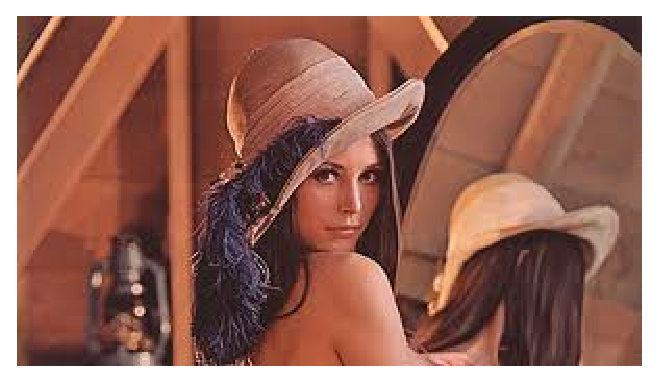
\includegraphics[scale=0.7]{Misc/TODO}
        \caption{}
        \label{Fig:3:RetrofittedLKFits}
    \end{center}
\end{figure}
%%
Table\ref{Tab:3:DingleTerms} lists the extracted Dingle terms for each peak of the Fermi surface.

\subsubsection{`Microfitting' the LK formula}

A second attempt at refining the LK fits was performed by applying the microfit technique desribed in section~\ref{Sec:2:LKMicrofitting}. $1.5$ oscillations were fit at a time Filtering the data beforehand is not always straightforward due to close proximity of neighbouring peaks. The stronger peaks from the $\alpha$ and $\beta$ Fermi surfaces show banding of the masses and a clear trending of the results to one of a few values which have been highlighted in yellow. Data in these regions were averaged to give the values in table \ref{Table:3:MicroFitResults}.

All filtered using function $\textit{F_{\textrm{filt}}}(x) = \textit{F}(x)/2 (\tanh{\pi(x - x_{\textrm{low}})/w} + \tanh{-\pi(x - x_{\textrm{high}})/w}$ where $\textit{F}$ is the Fourier transform of the torque data, $x$ is the dHvA frequency, $x_{\textrm{low}}$ and $x_{\textrm{high}}$ are the lower and upper limits of the filter range respectively and $w$ determines the trail off slope of the filter function. For all measurements $w=10$.
%%
\begin{figure}[h!]
    \begin{center}
        \includegraphics[scale=0.7]{Chapter3-dHvABaFe2P2/Figures/Mass/MicroFits/MicroFits}
        \caption{Effective temperature dependant masses extracted from fits to between one and three dHvA oscillations in the measured data. See Appendix\ref{Appendix:MicroFitParams} for a full list of parameters for each set of fits.}
        \label{Fig:3:MicroFits}
    \end{center}
\end{figure}
%%
\begin{center}
    \begin{tabular}[!h]{llllllll}
\toprule
Angle	& dHvA Freq. (\unit{T})	& Label	 & Upper Limit	& Lower	Limit	& Average $m^*_T$	& Stdev $m^*_T$	& Filter Width\\
\midrule
12	& 1210	& $\alpha_1$	& 17.0	& 11.0	& 1.75	& 0.03 &	1100--1240\\
28	& 1269	& $\alpha_1$	& 17.0	& 11.0	& 1.72	& 0.02 &	1200--1310\\
46	& 1532	& $\alpha_1$	& 17.0	& 9.0	& 1.92	& 0.02 &	1430--1585\\
12	& 1372	& $\alpha_2$	& 17.0	& 8.0	& 1.57	& 0.01 &	1320--1440\\
28	& 1530	& $\alpha_2$	& 17.0	& 8.0	& 1.75	& 0.02 &	1450--1650\\
46	& 2017	& $\alpha_2$	& 16.8	& 10.5	& 2.55	& 0.11 &	1970--2100\\
28	& 1365	& $\alpha_3$	& 17.0	& 9.5	& 1.97	& 0.03 &	1320--1440\\
46	& 1930	& $\alpha_3$	& 17.0	& 10.7	& 2.75	& 0.24 &	1890--1970\\
12	& 2180	& $\beta_1$	& 17.0	& 8.0	& 1.63	& 0.02 &	2100--2270\\
12	& 2350	& $\beta_2$	& 17.0	& 9.0	& 1.57	& 0.03 &	2270--2450\\
28	& 2605	& $\beta_2$	& 17.0	& 8.5	& 1.81	& 0.02 &	2555--2670\\
46	& 3347	& $\beta_2$	& 17.3	& 10.0	& 2.86	& 0.08 &	3250--3370\\
46	& 3381	& $\beta_2$	& 17.3	& 10.0	& 2.78	& 0.32 &	3365--2500\\
28	& 2475	& $\beta_3$	& 17.0	& 8.0	& 1.59	& 0.02 &	2400--2560\\
46	& 2970	& $\beta_3$	& 17.0	& 8.5	& 1.86	& 0.01 &	2850--3100\\
12	& 1270	& $\delta$	& 17.0	& 12.0	& 1.71	& 0.01 &	1250--1310\\
46	& 1626	& $\delta$	& 17.0	& 10.5	& 2.17	& 0.15 &	1590--1690\\
28	& 912	& $\gamma_1$	& 16.8	& 11.3	& 2.17	& 0.18 &	850--970  \\
46	& 1320	& $\gamma_1$	& 16.8	& 11.3	& 2.00	& 0.37 &	1270--1370\\
46	& 4497	& $\gamma_2$	& 16.8	& 12.2	& 3.31	& 0.13 &	4400--4600\\
\bottomrule
    \end{tabular}
    \label{Table:3:MicroFitResults}
    \caption{}
\end{center}

\subsection{Effective mass results}

Table~\ref{Table:3:EffectiveMasses} lists the results of the effective mass investigations.
%%
\medskip
%%TODO
\begin{center}
    \begin{tabular}[h!]{llr}
\toprule
Band    & \multicolumn{2}{l}{Energy Shift (\unit{Ry})} \\
\midrule
1       &       & -0.0083      \\
2       & Wide  & 0.0          \\
        & Narrow & -0.0038     \\
3       &       & 0.0043       \\
4       &       & 0.0050        \\
\bottomrule
    \label{Table:3:EnergyShifts}
    \end{tabular}
\end{center}

